\chapter{The MITIP, an atmospheric correction and image processing method}

\label{Chapter3}

%description
%----------------------------------------------------------------------------------------
This chapter gives a brief description about the MITIP method which is an atmospheric correction and image processing method for the TET-1 imagery, developed by Dr. Rudolf at DLR. Data preparation and pre-processing is given in Section 3.1. The processing procedure is descirbed briefly in Section 3.2. The output of MITIP is presented in Section 3.3.\\

%----------------------------------------------------------------------------------------
%	SECTION 1
%----------------------------------------------------------------------------------------

\section{Data preparation and pre-processing}

%-----------------------------------
%	SUBSECTION 1
%-----------------------------------

\subsection{Data preparation}
The TET-1 imagery input to the MITIP is radiometrically calibrated top-of-atmosphere (TOA) radiance data (Level 1B). In order to acquire ground surface radiance and temperature, atmospheric correction should be performed first.\\

\noindent The necessary atmospheric correction takes advantage of the fact that in the thermal spectral range water vapor is the dominating disturbing parameter, while aerosols play only a negligible role \parencite{Reference204}. Consequently, for the purpose of simplifying the procedure, water vapor is the only parameter that taken into account while performing atmosphric correction. Because it is impossible to retrieval of information of water vapor from TET-1 imagery, external data is required. MODIS water vapor products are used here. Besides, since the water vapor column decreases with elevation, the other parameter that has to included is the elevation, which is obtained from ASTER Digital Elevation Map (DEM).\\

\noindent From Chapter 2 we know, emissivity map needs to feed to MITIP to convert the derived radiant temperature $T_{rad}$ to kinetic temperature $T_{kin}$. The emissivity map can be acquired from ASTER Global Emissivity Database (GED).\\

\noindent Finally, the input files to the MITIP are:
\begin{itemize}
\item TET-1 imagery with TOA radiance
\item Water vapor from MODIS water vapor product
\item Elevation from ASTER Global Elevation Map
\item Emissivity map from ASTER Global Emissivity Database
\end{itemize}

\noindent All the auxiliary data can be downloaded from the website of NASA (National Aeronautics and Space Administration).\\

%-----------------------------------
%	SUBSECTION 2
%-----------------------------------

\subsection{Data pre-processing}
According to the MITIP's requirements, the input data should fulfill three conditions: 1) all input data should be of format GeoTIFF; 2) all input imageries should be overlapped and of the same size; 3) spatial resolution of all imageries should be identical.\\

\noindent As a result, after downloading all the auxiliary data, they should be converted into GeoTIFF format first. Then, compared with TET-1 imagery, the individual raster file of both the ASTER data has a smaller ground coverage which is arond 60 km by 60 km. These small raster files of ASTER DEM and GED should be merged into one large files respectively which are able to cover the whole area of interest (AOI). Next, to ensure all the four input files are overlapped with each other, they ought to be reprojected into the same and appropriate UTM zone and resampling to the same pixel size. Finally, the TET-1 imagery is used as standard defining the size of the input file. All input data should be clipped using TET-1 imagery as mask to guarantee they all share the same number of rows and columns.\\ 

%----------------------------------------------------------------------------------------
%	SECTION 2
%----------------------------------------------------------------------------------------

\section{Procedure of the MITIP}

The radiative transfer function in the thermal region can be expressed as:
\begin{equation}
\begin{aligned}
\label{eq301}
L(\lambda) = L_p(\lambda) + \tau (\lambda) \varepsilon (\lambda) L_{bb}(\lambda, T) + \tau (\lambda) (1 - \varepsilon (\lambda)) \frac{F(\lambda)}{\pi}\\
+L_{p,s}(\lambda) + \frac{\tau (\lambda) E_g(\lambda) \frac{\rho (\lambda)}{\pi}}{1 - \rho (\lambda) s(\lambda)}
\end{aligned}
\end{equation}

\noindent with:\\
\indent $L(\lambda)$: at-sensor radiance\\
\indent $L_p(\lambda)$: thermal path radiance\\
\indent $\tau (\lambda)$: ground-to-sensor atmospheric transmittance\\
\indent $\varepsilon (\lambda)$: emissivity\\
\indent $L_{bb}(\lambda, T)$: blackbody radiance at the ground surface\\
\indent $F(\lambda)$: thermal downwelling flux on the ground\\
\indent $L_{p, s}(\lambda)$: solar scattered path radiance\\
\indent $E_g(\lambda)$: global (direct + diffuse) solar flux on the ground\\
\indent $s(\lambda)$: spherical albedo\\
\indent $\rho (\lambda)$: surface reflectance\\

\noindent As most objects are opaque and do not transmit radiation, we have:
\begin{equation}
\label{eq302}
\rho (\lambda) = 1 - \varepsilon (\lambda)
\end{equation}

\noindent The first line of Equation \eqref{eq301} describes the thermal components and the second line the solar radiation. Since in this thesis we restrict ourselves to the night-time TET-1 scenes, the radiative transfer function for the MIR and TIR bands of TET-1 imagery is
\begin{equation}
\label{eq303}
L(\lambda) = L_p(\lambda) + \tau (\lambda) \varepsilon (\lambda) L_{bb}(\lambda, T) + \tau (\lambda) (1 - \varepsilon (\lambda)) \frac{F(\lambda)}{\pi}
\end{equation}

\noindent Multiplying both sides of Equation \eqref{eq303} with the channel spectral response function $R(\lambda)$ and integrating over the bandpass field we have:
\begin{equation}
\label{eq304}
L(k) = L_p(k) + \tau (k) \varepsilon (k) L_{bb}(k, T) + \tau (k) (1 - \varepsilon (k)) \frac{F(k)}{\pi}
\end{equation}

\noindent with:\\
\indent $k$ = band number; $k$ = 1: MIR, $k$ = 2: TIR\\

In most cases of interest to fire detection, the 3 - 5 $\mu$m surface emissivity is between 0.75 - 1.0 \parencite{Reference301}, while the 8 - 12 $\mu$m emissivity is between 0.95 - 1.0 \parencite{Reference302}, as showed in Figure \ref{fig:emi_soil}, \ref{fig:emi_vegetation} and \ref{fig:emi_water}.\\

\begin{figure}[!htbp]
  \centering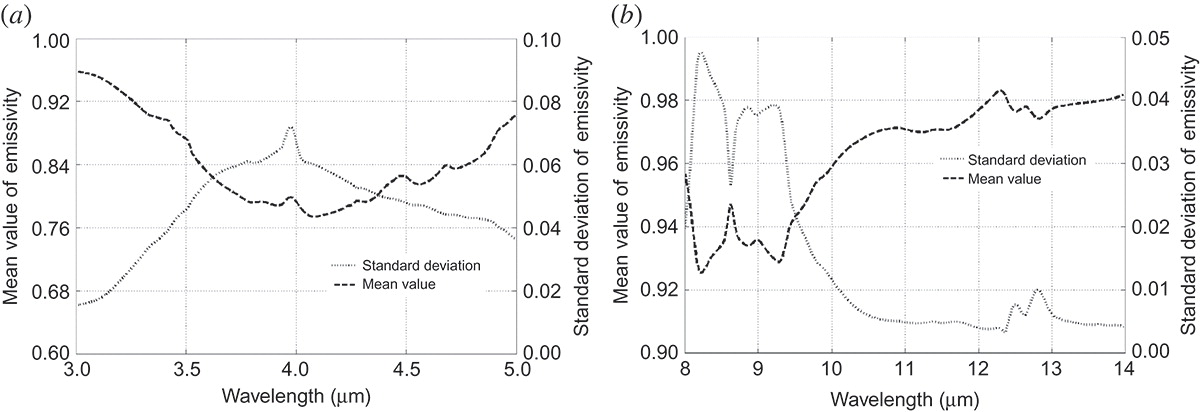
\includegraphics[width=0.9\textwidth]{emi_soil.jpeg}
  \caption{Emissivity spectra for soils in the ASTER spectral emissivity database. (a) 3 - 5 $\mu$m. (b) 8 - 14 $\mu$m. \parencite{Reference303}.}
  \label{fig:emi_soil}
  
  \centering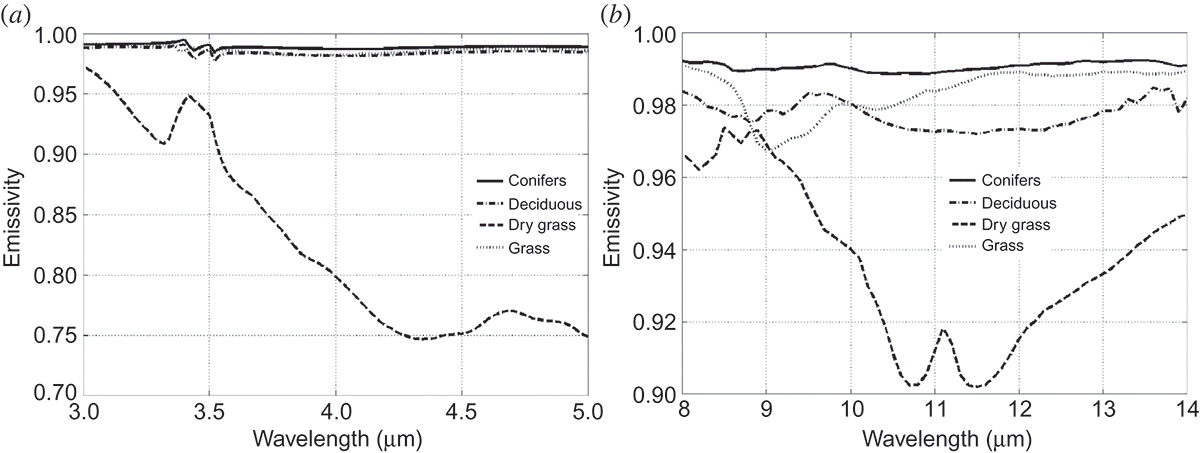
\includegraphics[width=0.9\textwidth]{emi_vegetation.jpeg}
  \caption{Emissivity spectra for four types of vegetation in the ASTER spectral emissivity database. (a) 3 - 5 $\mu$m. (b) 8 - 14 $\mu$m. \parencite{Reference303}.}
  \label{fig:emi_vegetation}
  
  \centering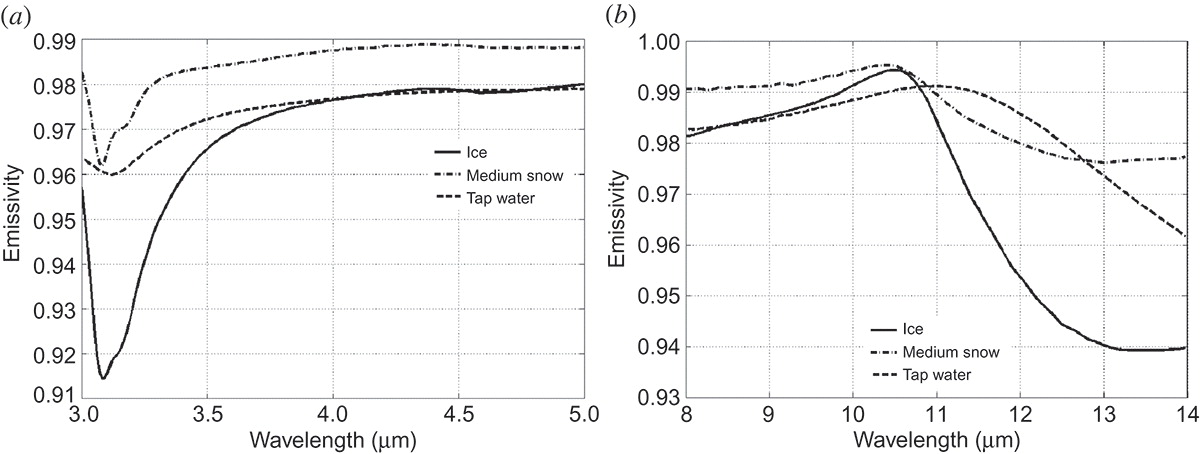
\includegraphics[width=0.9\textwidth]{emi_water.jpeg}
  \caption{Emissivity spectra for water, ice and snow in the ASTER spectral emissivity database. (a) 3 - 5 $\mu$m. (b) 8 - 14 $\mu$m. \parencite{Reference303}.}
  \label{fig:emi_water}
\end{figure}

\noindent Denote hte product $\varepsilon(k) L_{bb}(k, T) = L_{surf}^*(k, T)$ as the ''effective'' or ''radiative'' surface radiance, we can get:
\begin{equation}
\label{eq305}
L_{surf}^*(k, T) = \frac{L(k) - L_p(k)}{\tau (k)} - (1 - \varepsilon (k)) \frac{F(k)}{\pi}
\end{equation}

\noindent Considering in both MIR and TIR band the emissivity is close to 1, so the term $1 - \varepsilon (k)$ will be a small term so that the thermal downwelling flux term $F(k)$ will have only a small influence. Finally, all the terms $L_p(k)$, $F(k)$ and $\tau (k)$ will be calculated by MODTRAN (MODerate resolution atmospheric TRANsmission) as a function of atmospheric water vapor volumn $W(e)$, $W$ for short, which acts as a function of elevation $e$, for MIR and TIR band of TET-1 imagery respectively.\\

\noindent Finally, the surface radiance of both the black body and natural materials can be calculated from Equation \eqref{eq305}. The atmospheric correction for the night-time TET-1 scenes are done.\\

\noindent With the help of Planck's function and its inversion, surface temperature for the MIR and TIR band of TET-1 imagery can be derived. Using the dual-channel method proposed by Matson and Dozier (1981), the final HTE monitoring products including effective target temperature $T_t$, effective target pixel fraction and Fire Radiative Power (FRP) can be obtained.\\

%----------------------------------------------------------------------------------------
%	SECTION 3
%----------------------------------------------------------------------------------------

\section{Outcomes of the MITIP}
The outcomes of MITIP can be classified into two parts: one part is the result of atmospheric and another the HTE monitoring product.